\documentclass{article}
\usepackage{tikz}
\usetikzlibrary{positioning, arrows.meta, calc}

\begin{document}

\begin{figure}
\centering
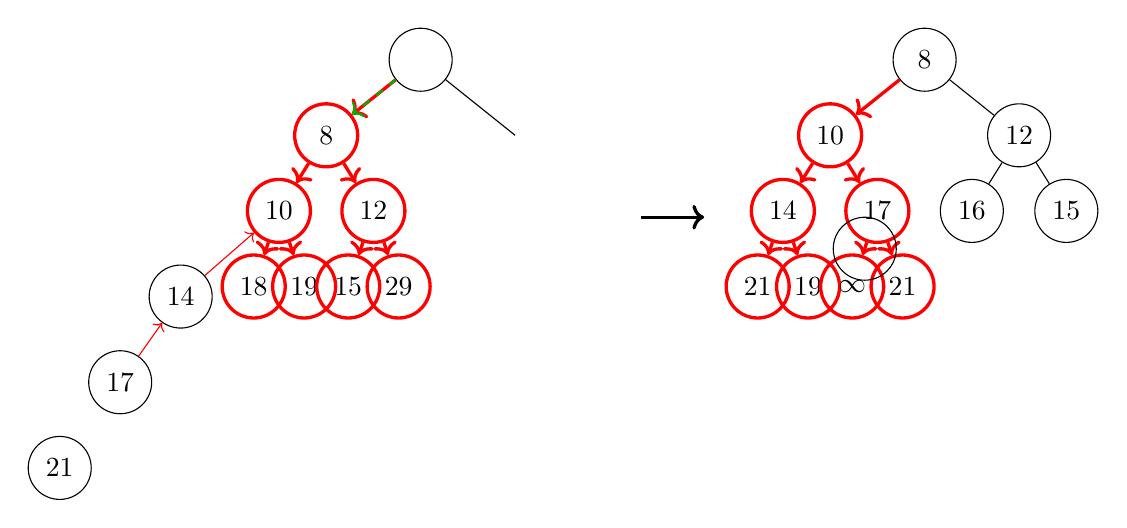
\begin{tikzpicture}[
  scale=0.8,
  level distance=1.2cm,
  every node/.style={circle,draw,minimum size=8mm,inner sep=0pt},
  level 1/.style={sibling distance=30mm},
  level 2/.style={sibling distance=15mm},
  level 3/.style={sibling distance=8mm},
  rededge/.style={draw=red, very thick, ->},
  graynode/.style={fill=gray!30}
]

% Left tree (before)
\node (n0) {}
  child[rededge] {node (n1) {8}
    child[rededge] {node (n2) {10}
      child {node {18}}
      child {node {19}}
    }
    child {node (n3) {12}
      child {node {15}}
      child {node {29}}
    }
  }
  child[draw=none] {};

% Left deeper levels
\path (n2) -- ++(-1.2,-1) node[below left] (n4) {14}
      (n4) edge[red,->] (n2)
      (n4) -- ++(-.6,-1) node[below left] (n5) {17}
      (n5) edge[red,->] (n4)
      (n5) -- ++(-.6,-1) node[below left] (n6) {21};

% Dashed green edge for insertion
\draw[->, thick, dashed, green!70!black] (n0) -- (n1);

% Right tree (after)
\begin{scope}[xshift=8cm]
\node (m1) {8}
  child[rededge] {node (m2) {10}
    child[rededge] {node (m3) {14}
      child {node {21}}
      child {node {19}}
    }
    child[rededge] {node (m4) {17}
      child[graynode] {node {$\infty$}}
      child {node {21}}
    }
  }
  child {node (m5) {12}
    child {node {16}}
    child {node {15}}
  };
\node at ($(m4)!0.5!(m4-1)$) {};
\end{scope}

% Arrow between trees
\draw[very thick,->] (3.5,-2.5) -- (4.5,-2.5);

\end{tikzpicture}
\caption{Heap after insertion of 7 and reheapification.}
\end{figure}

\end{document}
